\begin{pastexam}[label={px:gk3-115-ds-03}]{高考三級資訊處理 115 年 第三題}
（申論；25 分）

給定一棵二元搜尋樹（binary search tree），且該樹同時也是一棵 AVL 樹。樹的節點在 C 語言中宣告如下：
\begin{minted}[fontsize=\small]{c}
typedef struct Node {
    int key;             // 節點的鍵值，所有節點的鍵值皆互不相同
    int size;            // 以該節點為根的子樹節點總數 (包含自己)
    struct Node *left;   // 指向左子節點
    struct Node *right;  // 指向右子節點
} Node;
\end{minted}
並定義以下函式：

int size (Node *$node$)：\\
\hspace*{1.5em}若傳入的 $node$ 為 NULL，則回傳 0；否則回傳 $node$ -> size。\\
int count\_less\_equal (Node *$node$, int $val$)：\\
\hspace*{1.5em}回傳以 $node$ 為根的子樹中，所有鍵值小於等於 $val$ 的節點總數。\\
Node* select (Node *$node$, int $r$)：\\
\hspace*{1.5em}回傳以 $node$ 為根的子樹中，第 $r$ 小的節點指標，$r$ 從 1 開始算。\\
Node* greater\_k\_smallest (Node *$root$, int $val$, int $k$)：\\
\hspace*{1.5em}找出以 $root$ 為根的整棵樹中，所有鍵值大於 $val$ 的節點裡，第 $k$ 小的節點，$k$ 從 1 開始算。若第
$k$ 小的節點不存在，則回傳 NULL。
\begin{itemize}[leftmargin=2.2em]
\item[㈠] 完成下列程式碼的空格。（20 分）
\begin{minted}[fontsize=\small,escapeinside=@@]{c}
int count_less_equal(Node *node, int val) {
    if (node == NULL) return 0;
    if (node->key > val)
        return count_less_equal(node->left, val);
    else return size(node->left)+ @\blank{1}@;
}
Node* select(Node *node, int r) {
    int left_size = size(node->left);
    if (r == @\blank{2}@) return node;
    else if (r <= left_size)
        return select(node->left, r);
    else return @\blank{3}@;
}
Node* greater_k_smallest(Node *root, int val, int k){
    int x = count_less_equal(root, val);
    int y = @\blank{4}@;
    if (y > size(root)) return NULL;
    return select(root, y);
}
\end{minted}
\item[㈡] 下圖為一棵包含 5 個節點且滿足 AVL 平衡特性的二元搜尋樹，圖中顯示每個節點的鍵值。若將鍵值為 70 的
新節點插入此樹，為保持 AVL 樹的平衡，會觸發旋轉。請畫出旋轉後的樹狀結構圖。除新插入的節點 70 外，若原有節點
的 size 欄位值在旋轉後發生改變，請在旋轉後的圖中，於該節點旁標示其新的 size 欄位值。（5 分）
\begin{center}
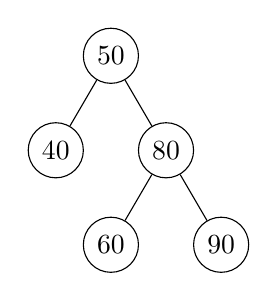
\begin{tikzpicture}[v/.style={circle,draw,minimum size=7mm,inner sep=0pt},
  level distance=12mm, level 1/.style={sibling distance=14mm}, level 2/.style={sibling distance=14mm}]
\node[v] {50}
  child {node[v] {40}}
  child {node[v] {80} child {node[v] {60}} child {node[v] {90}}};
\end{tikzpicture}
\end{center}
\end{itemize}
\end{pastexam}

\begin{pastsoln}
答案：㈠ (1) \texttt{1 + count\_less\_equal(node->right, val)}；(2) \texttt{left\_size + 1}；
(3) \texttt{select(node->right, r - left\_size - 1)}；(4) \texttt{x + k}。 ㈡ 右左（RL）雙旋轉，$60$ 成為根，
左子樹 $50$（左子 $40$），右子樹 $80$（左子 $70$、右子 $90$）；size 改變的是 $60$（變 $6$）和 $50$（變 $2$）。
㈠ 屬資結書第~9.4~節（順序統計），㈡ 屬第~10.2~節（AVL 插入）。

\textbf{㈠} 這是資結書第~9.4~節的 rank 和 select，靠的是每個節點的 $\mathit{size}$ 欄位。
\begin{itemize}
\item \textbf{(1)}：若 \texttt{node->key <= val}，左子樹的鍵都比 \texttt{node->key} 小，全部 $\le$ val，共
\texttt{size(node->left)} 個；\texttt{node} 自己也算 $1$ 個；右子樹的鍵比 \texttt{node->key} 大，其中哪些 $\le$ val
不知道，要遞迴算。 所以填 \texttt{1 + count\_less\_equal(node->right, val)}。 （另一個分支：\texttt{node->key > val}
時，自己和整個右子樹都 $>$ val，只要算左子樹，這是題目已給的部分。）
\item \textbf{(2)}：左子樹有 \texttt{left\_size} 個比 \texttt{node} 小的鍵，所以 \texttt{node} 是這棵子樹第
\texttt{left\_size + 1} 小的。 填 \texttt{left\_size + 1}。
\item \textbf{(3)}：$r > \texttt{left\_size} + 1$，要找的在右子樹。 右子樹之前已經有左子樹的 \texttt{left\_size} 個和
\texttt{node} 自己 $1$ 個，所以在右子樹裡是第 $r - \texttt{left\_size} - 1$ 小。 填
\texttt{select(node->right, r - left\_size - 1)}。
\item \textbf{(4)}：整棵樹裡 $\le$ val 的有 $x$ 個，它們正好是第 $1$ 到第 $x$ 小（鍵值互不相同）。 $>$ val 的節點
是第 $x + 1, x + 2, \ldots$ 小，其中第 $k$ 小的就是整棵樹第 $x + k$ 小。 填 \texttt{x + k}。 接著的
\texttt{if (y > size(root)) return NULL;} 處理「大於 val 的節點不到 $k$ 個」。
\end{itemize}
三個函式每層只往下走一邊，花 $O(1)$，所以都是 $O(h)$；AVL 樹的 $h = O(\log n)$（資結書定理~10.1），
\texttt{greater\_k\_smallest} 是 $O(\log n)$。

小例子：㈡ 的原樹，val $= 55$、$k = 2$：\texttt{count\_less\_equal} 在 $50$ 走右邊得 $1 + 1 + \text{count}(80)$，
在 $80$ 走左邊、在 $60$ 走左邊得 $0$，所以 $x = 2$；$y = 4$，\texttt{select(root, 4)}：根的 left\_size $= 1$，
$4 > 2$，到右子樹找第 $4 - 1 - 1 = 2$ 小；$80$ 的 left\_size $= 1$，$2 = 1 + 1$，回傳 $80$。 大於 $55$ 的有
$60, 80, 90$，第 $2$ 小確實是 $80$。

\textbf{㈡} 插入 $70$：$70 > 50$ 往右，$70 < 80$ 往左，$70 > 60$，成為 $60$ 的右子節點。 沿路往上檢查高度（葉子
高度記 $1$）：$60$ 的高度變 $2$，$80$ 左高 $2$、右高 $1$，平衡因子 $+1$ 還可以；$50$ 左高 $1$、右高 $3$，平衡
因子 $-2$，失衡。 新節點在 $50$ 的\textbf{右}子節點（$80$）的\textbf{左}子樹，是 \textbf{RL 型}，做雙旋轉
（資結書第~10.2.3~節）：先對 $80$ 右旋（$60$ 上來），再對 $50$ 左旋（$60$ 成為這棵子樹的根）。 $60$ 原本的
左子樹（空）給 $50$ 當右子樹，右子樹 $\{70\}$ 給 $80$ 當左子樹。
\begin{center}
\begin{tikzpicture}[v/.style={circle,draw,minimum size=7mm,inner sep=0pt},
  s/.style={font=\small,text=examStroke!70!black},
  level distance=12mm, level 1/.style={sibling distance=26mm}, level 2/.style={sibling distance=14mm}]
\node[v] (r) {60}
  child {node[v] (a) {50} child {node[v] {40}} child[missing] {}}
  child {node[v] (b) {80} child {node[v] {70}} child {node[v] {90}}};
\node[s,right=1mm of r] {size $= 6$};
\node[s,left=1mm of a] {size $= 2$};
\end{tikzpicture}
\end{center}
各節點的 size：
\begin{center}
\small
\begin{tabular}{lccc}
\toprule
節點 & 原樹（插入前） & 旋轉後 & 是否改變 \\
\midrule
60 & 1 & 6 & 是 \\
50 & 5 & 2 & 是 \\
80 & 3 & 3 & 否 \\
40, 90 & 1 & 1 & 否 \\
\bottomrule
\end{tabular}
\end{center}
所以圖中標出 $60$ 的新 size $6$、$50$ 的新 size $2$。 （$80$ 在插入 $70$ 之後、旋轉之前曾暫時是 $4$，旋轉後子樹是
$\{70, 80, 90\}$，又回到 $3$，和原樹相同，不必標。 如果把「旋轉前」理解為插入後尚未旋轉的狀態，$80$ 也從 $4$
變成 $3$，可以一併標上。）旋轉時只有參與旋轉的節點要重算 size，依「先子後父」的順序用
$\mathit{size} = \mathit{size}(\mathit{left}) + \mathit{size}(\mathit{right}) + 1$ 更新即可，每次旋轉 $O(1)$。
\end{pastsoln}
